%%% File-Information {{{
%%% Filename: template_bericht.tex
%%% Purpose: lab report, technical report, project report
%%% Time-stamp: <2004-06-30 18:19:32 mp>
%%% Authors: The LaTeX@TUG-Team [http://latex.tugraz.at/]:
%%%          Karl Voit (vk), Michael Prokop (mp), Stefan Sollerer (ss)
%%% History:
%%%   20050914 (ss) correction of "backref=true" to "backref" due to hyperref documentation
%%%   20040630 (mp) added comments to foldmethod at end of file
%%%   20040625 (vk,ss) initial version
%%%
%%% Notes:
%%%
%%%
%%%
%%% }}}
%%%%%%%%%%%%%%%%%%%%%%%%%%%%%%%%%%%%%%%%%%%%%%%%%%%%%%%%%%%%%%%%%%%%%%%%%%%%%%%%
%%% main document {{{

\documentclass[
a4paper,     %% defines the paper size: a4paper (default), a5paper, letterpaper, ...
% landscape,   %% sets the orientation to landscape
% twoside,     %% changes to a two-page-layout (alternatively: oneside)
% twocolumn,   %% changes to a two-column-layout
% headsepline, %% add a horizontal line below the column title
% footsepline, %% add a horizontal line above the page footer
% titlepage,   %% only the titlepage (using titlepage-environment) appears on the first page (alternatively: notitlepage)
% parskip,     %% insert an empty line between two paragraphs (alternatively: halfparskip, ...)
% leqno,       %% equation numbers left (instead of right)
% fleqn,       %% equation left-justified (instead of centered)
% tablecaptionabove, %% captions of tables are above the tables (alternatively: tablecaptionbelow)
% draft,       %% produce only a draft version (mark lines that need manual edition and don't show graphics)
% 10pt         %% set default font size to 10 point
% 11pt         %% set default font size to 11 point
12pt         %% set default font size to 12 point
]{scrartcl}  %% article, see KOMA documentation (scrguide.dvi)



%%%%%%%%%%%%%%%%%%%%%%%%%%%%%%%%%%%%%%%%%%%%%%%%%%%%%%%%%%%%%%%%%%%%%%%%%%%%%%%%
%%%
%%% packages
%%%

%%%
%%% encoding and language set
%%%

%%% ngerman: language set to new-german
%\usepackage{ngerman}
\usepackage[english]{babel}

%%% babel: language set (can cause some conflicts with package ngerman)
%%%        use it only for multi-language documents or non-german ones
%\usepackage[ngerman]{babel}

%%% inputenc: coding of german special characters
\usepackage[utf8]{inputenc}

%%% fontenc, ae, aecompl: coding of characters in PDF documents
\usepackage[T1]{fontenc}
\usepackage{ae,aecompl}

%%%
%%% technical packages
%%%

%%% amsmath, amssymb, amstext: support for mathematics
%\usepackage{amsmath,amssymb,amstext}

%%% psfrag: replace PostScript fonts
\usepackage{psfrag}

%%% listings: include programming code
%\usepackage{listings}

%%% units: technical units
%\usepackage{units}

%%%
%%% layout
%%%

%%% scrpage2: KOMA heading and footer
%%% Note: if you don't use this package, please remove 
%%%       \pagestyle{scrheadings} and corresponding settings
%%%       below too.
\usepackage[automark]{scrpage2}

%%%
%%% BibLaTeX
%%%

\usepackage[backend=biber, %% Hilfsprogramm "biber" (statt "biblatex" oder "bibtex")
style=authoryear, %% Zitierstil (siehe Dokumentation)
natbib=true, %% Bereitstellen von natbib-kompatiblen Zitierkommandos
hyperref=true, %% hyperref-Paket verwenden, um Links zu erstellen
]{biblatex}

\addbibresource{literature.bib} %% Einbinden der bib-Datei

%%%
%%% PDF
%%%

\usepackage{ifpdf}

%%% Should be LAST usepackage-call!
%%% For docu on that, see reference on package ``hyperref''
\ifpdf%   (definitions for using pdflatex instead of latex)

  %%% graphicx: support for graphics
  \usepackage[pdftex]{graphicx}

  \pdfcompresslevel=9

  %%% hyperref (hyperlinks in PDF): for more options or more detailed
  %%%          explanations, see the documentation of the hyperref-package
  \usepackage[%
    %%% general options
    pdftex=true,      %% sets up hyperref for use with the pdftex program
    %plainpages=false, %% set it to false, if pdflatex complains: ``destination with same identifier already exists''
    %
    %%% extension options
    backref,      %% adds a backlink text to the end of each item in the bibliography
    pagebackref=false, %% if true, creates backward references as a list of page numbers in the bibliography
    colorlinks=true,   %% turn on colored links (true is better for on-screen reading, false is better for printout versions)
    %
    %%% PDF-specific display options
    bookmarks=true,          %% if true, generate PDF bookmarks (requires two passes of pdflatex)
    bookmarksopen=false,     %% if true, show all PDF bookmarks expanded
    bookmarksnumbered=false, %% if true, add the section numbers to the bookmarks
    %pdfstartpage={1},        %% determines, on which page the PDF file is opened
    pdfpagemode=None         %% None, UseOutlines (=show bookmarks), UseThumbs (show thumbnails), FullScreen
  ]{hyperref}


  %%% provide all graphics (also) in this format, so you don't have
  %%% to add the file extensions to the \includegraphics-command
  %%% and/or you don't have to distinguish between generating
  %%% dvi/ps (through latex) and pdf (through pdflatex)
  \DeclareGraphicsExtensions{.pdf}

\else %else   (definitions for using latex instead of pdflatex)

  \usepackage[dvips]{graphicx}

  \DeclareGraphicsExtensions{.eps}

  \usepackage[%
    dvips,           %% sets up hyperref for use with the dvips driver
    colorlinks=false %% better for printout version; almost every hyperref-extension is eliminated by using dvips
  ]{hyperref}

\fi


%%% sets the PDF-Information options
%%% (see fields in Acrobat Reader: ``File -> Document properties -> Summary'')
%%% Note: this method is better than as options of the hyperref-package (options are expanded correctly)
\hypersetup{
  pdftitle={}, %%
  pdfauthor={}, %%
  pdfsubject={}, %%
  pdfcreator={Accomplished with LaTeX2e and pdfLaTeX with hyperref-package.}, %% 
  pdfproducer={}, %%
  pdfkeywords={} %%
}


%%%%%%%%%%%%%%%%%%%%%%%%%%%%%%%%%%%%%%%%%%%%%%%%%%%%%%%%%%%%%%%%%%%%%%%%%%%%%%%%
%%%
%%% user defined commands
%%%

%%% \mygraphics{}{}{}
%% usage:   \mygraphics{width}{filename_without_extension}{caption}
%% example: \mygraphics{0.7\textwidth}{rolling_grandma}{This is my grandmother on inlinescates}
%% requires: package graphicx
%% provides: including centered pictures/graphics with a boldfaced caption below
%% 
\newcommand{\mygraphics}[3]{
  \begin{center}
    \includegraphics[width=#1, keepaspectratio=true]{#2} \\
    \textbf{#3}
  \end{center}
}

\usepackage{booktabs}

%%%%%%%%%%%%%%%%%%%%%%%%%%%%%%%%%%%%%%%%%%%%%%%%%%%%%%%%%%%%%%%%%%%%%%%%%%%%%%%%
%%%
%%% define the titlepage
%%%

% \subject{}   %% subject which appears above titlehead
% \titlehead{} %% special heading for the titlepage

%%% title
\title{Introduction into bipartite networks with Python}

\subtitle{Networks Seminar at Karl Franzens University of Graz, Peter Csermely}

%%% author(s)
\author{Stefan Kasberger (1011416)}

%%% date
\date{Graz, on \today{}}

% \publishers{}

% \thanks{} %% use it instead of footnotes (only on titlepage)

% \dedication{} %% generates a dedication-page after titlepage


%%% uncomment following lines, if you want to:
%%% reuse the maketitle-entries for hyperref-setup
%\newcommand\org@maketitle{}
%\let\org@maketitle\maketitle
%\def\maketitle{%
%  \hypersetup{
%    pdftitle={\@title},
%    pdfauthor={\@author}
%    pdfsubject={\@subject}
%  }%
%  \org@maketitle
%}


%%%%%%%%%%%%%%%%%%%%%%%%%%%%%%%%%%%%%%%%%%%%%%%%%%%%%%%%%%%%%%%%%%%%%%%%%%%%%%%%
%%%
%%% set heading and footer
%%%

%%% scrheadings default: 
%%%      footer - middle: page number
\pagestyle{scrheadings}

%%% user specific
%%% usage:
%%% \position[heading/footer for the titlepage]{heading/footer for the rest of the document}

%%% heading - left
% \ihead[]{}

%%% heading - center
% \chead[]{}

%%% heading - right
% \ohead[]{}

%%% footer - left
% \ifoot[]{}

%%% footer - center
% \cfoot[]{}

%%% footer - right
% \ofoot[]{}



%%%%%%%%%%%%%%%%%%%%%%%%%%%%%%%%%%%%%%%%%%%%%%%%%%%%%%%%%%%%%%%%%%%%%%%%%%%%%%%%
%%%
%%% begin document
%%%

\begin{document}

% \pagenumbering{roman} %% small roman page numbers

%%% include the title
% \thispagestyle{empty}  %% no header/footer (only) on this page

\maketitle

%%% start a new page and display the table of contents
% \newpage
% \tableofcontents

%%% start a new page and display the list of figures
% \newpage
% \listoffigures

%%% start a new page and display the list of tables
% \newpage
% \listoftables

%%% display the main document on a new page 
% \newpage

% \pagenumbering{arabic} %% normal page numbers (include it, if roman was used above)

%%%%%%%%%%%%%%%%%%%%%%%%%%%%%%%%%%%%%%%%%%%%%%%%%%%%%%%%%%%%%%%%%%%%%%%%%%%%%%%%
%%%
%%% begin main document
%%% structure: \section \subsection \subsubsection \paragraph \subparagraph
%%%


%%%%%%%%%%%%%%%%%%
%  INTRODUCTION  %
%%%%%%%%%%%%%%%%%%

\section{Introduction}
\label{sec:introduction}

This essay and the related computation delivers a comprehensive introduction into the concept of bipartite networks, a class of networks whose nodes are divided into two sets and only the connection between two nodes in different sets is allowed \citep{easley_networks_2010}. The analysis and visualization is done in the programming language Python and offers easy to understand first steps in both fields, network analyses and python programming. As data a collaboration network of github users and projects and an affiliation network of dbpedia entities with countries from KONECT are used. 
The analysis compares key measures like average shortest path, density, degree centrality and clustering. Also the topic of bipartite network projections to unipartite ones will be addressed on a practical and theoretical level. A specialty is, that the whole documentation and computation is done the open way in use of the Open Source Softwares LaTeX, Python and Git/GitHub to make it reproducible, freely accessible and useable for everyone.

%%%%%%%%%%%%
%  THEORY  %
%%%%%%%%%%%%

\section{Theory}
\label{sec:theory}

The theoretical basis for networks is the graph theory. By definition, a graph is a way of specifying relationships among a collection of items. It consists of a set of objects, called nodes, with certain pairs of these objects connected by links called edges \citep{easley_networks_2010}. Because of this flexible formalism, it is easy to find networks in many domains, like social sciences, micro-biology, psychology and engineering.

Different types of networks exist, depending on their structure and properties. Edges can be directed, from one node to another with a certain direction, or undirected, which means the relation is working in both directions and is symmetric. Typical undirected networks are links on webpages. Friendships for example are mostly undireced. The edges also can be weighted to give the relation a quantifiable dimension, like how often you met each other before or how big the bandwidth of a transmission channel is.\\

This article focuses on bipartite networks: A particular class of networks, whose nodes are divided into two sets, X and Y, and only the connection between two nodes in different sets is allowed \citep{easley_networks_2010}. Nodes from set X are only connected with nodes from set Y, not with other nodes from X, and vice versa. The connections can be weighted/unweighted or directed/undirected.

\begin{figure}[h!]
  \centering
  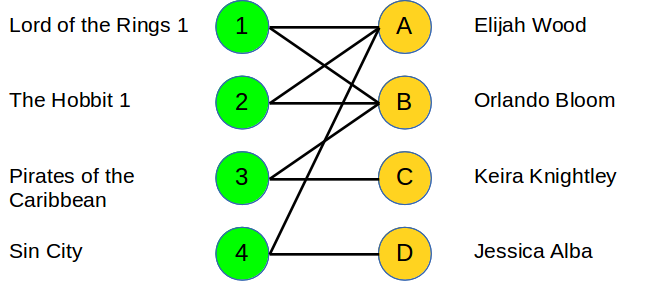
\includegraphics[width=0.7\textwidth]{./images/bipartite-actor-movie.png}
  \caption{Actor-movie bipartite network. Green nodes are movie nodes, yellow ones are actor nodes.}
  \label{fig:bipartite-network}
\end{figure}

In order to show the direct relations among a particular set of nodes \citep{zhou_how_2007}, because of the lack of appropriate notions and tools to address bipartite networks and to compare a particular network to others, one generally transforms a bipartite network into its X- or Y-projection \citep{latapy_basic_2008}, only consisting of one type of nodes. This is shown best through an example. Let's take a bipartite network of actors (yellow) and movies (green) as shown in figure \ref{fig:bipartite-network}, which gets projected to an actor-actor unipartite network (figure \ref{fig:unipartite-network}). Actor-actor means, that the projection looks on the relations between actors through their connection to movies. When actor $x_{1}$ played with actor $x_{2}$, the nodes $x_{1}$ and $x_{2}$ get connected in the projected unipartite graph. This goes on as long as all actor-movie-actor paths were projected. The created unipartite network only exists of actors connected together, and the edges carry the information that the actors played together in a movie.

\begin{figure}[h!]
  \centering
  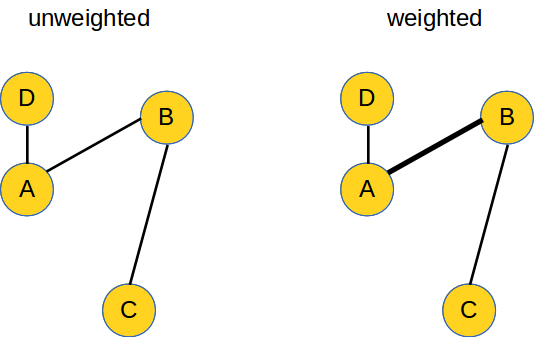
\includegraphics[width=0.5\textwidth]{./images/unipartite-actor-actor.png}
  \caption{Projected unipartite network from bipartite Actor-Movie network}
  \label{fig:unipartite-network}
\end{figure}

The projection, more precisely the information loss through it, leads to some serious problems. Some will be mentioned here: 1) It's lost if the actors played in more than one movie together, 2) the bipartite clustering coefficient differs from its unipartite counterpart and varies widely for given unipartite values, demonstrating the distinction between unipartite and bipartite embeddedness in the network \citep{piepenbrink_methodological_2013} and 3) in which movie(s) they played together and. The first problem is solved by the use of a weighted projection, where the resulting network carries the number of co-occurances as edge weight and the second can be tackled by looking at the clustering coefficient of the bipartite network. The last one is an unsolveable part of projections. Another blemish is, that the information contained by the edge whose adjacent X node (Y node) is of degree one, will be lost in X-projection (Y-projection) \citep{zhou_how_2007}. 
In sense of computation, the inflationary growth of edges through projection can cause troubles. Notice that each top node of degree $d$ induces links in the X-projection, and conversely \citep{latapy_basic_2008}. 
And empiricaly there are also issues: When the number of connections grow, the amount of interactions between the nodes normally decrease, but this information is lost through the projection. Generally this means, that the projection to unipartite networks ignores the possibility that bipartite networks have characteristics unique to their specific nature, which cannot be captured from a unipartite network perspective \citep{piepenbrink_methodological_2013}.

There are also specificities of the measurements. It is shown that the expected clustering coefficient in the projections is large, and give an efficient estimation formula; this means that a high clustering coefficient in a projection may be seen as a consequence of the underlying bipartite structure rather than a specific property of the network. Conversely, if the clustering coefficient of the projection is different from the expected one, it means that the underlying bipartite structure has nontrivial properties responsible for it (\cite{latapy_basic_2008}; \cite{newman_random_2001}; \cite{guillaume_bipartite_2004}; \cite{guillaume_bipartite_2006}).

In particular, there is a high heterogeneity between degrees of nodes of at least one kind, and there are significant overlaps between neighbourhoods \citep{latapy_basic_2008}.

%%%%%%%%%%%%%%%%%%%%%%%%%%%%%%
%  ANALYSIS & VISUALIZATION  %
%%%%%%%%%%%%%%%%%%%%%%%%%%%%%%

\section{Analysis and Visualization}
\label{sec:analysis-visualization-ipython}

\subsection{Data}
\label{sub:data}

The data used in this introduction is provided by the KONECT\footnote{\url{http://konect.uni-koblenz.de/}} project from the Web Science and Technology Institute (WeST)\footnote{\url{http://west.uni-koblenz.de/}} at the University of Koblenz-Landau.

\begin{itemize}
\item dbPedia \citep{konect:2014:dbpedia-country}: Relations between dbPedia\footnote{\url{http://dbpedia.org/About}} entities with countries, like Mozart lived in Austria.
\item GitHub \citep{konect:2014:github}: Collaboration-network of users and the projects they contributed to.
\end{itemize}

All KONECT data are licensed under a Creative Commons Attribution-ShareAlike 2.0 Germany License. \footnote{\url{https://creativecommons.org/licenses/by-sa/2.0/de/deed.en}}

\begin{flushleft}
  
\includegraphics[width=0.14\textwidth]{./images/cc-by-sa.png}
\end{flushleft}

\subsection{Reproducible Setup and Workflow}
\label{sub:reproducibility-workflow}

To be able to make the analysis reproducible, the process will be done openly, what is summarized under the term Open Science\footnote{\url{https://en.wikipedia.org/wiki/Open_science}}. Only Open Source Software\footnote{\url{https://en.wikipedia.org/wiki/Open-source_software}} were used together with Open Data Formats\footnote{\url{https://en.wikipedia.org/wiki/Open_format}}.
The whole computation and visualization is done with Python's\footnote{\url{http://www.python.org/}} iPython Notebook \citep{PER-GRA:2007}, an interactive scientific computing system in which source code and documentation can be written in one single document. Inside it, for the network analysis the module networkX\footnote{\url{http://networkx.github.io/}} is used and for plotting matplotlib \citep{Hunter:2007}. The iPython notebook is stored in a JSON\footnote{\url{http://www.json.org/}} file and can be exported easily in different formats like Markdown\footnote{\url{https://en.wikipedia.org/wiki/Markdown}}, PDF, HTML or TeX\footnote{\url{https://en.wikipedia.org/wiki/TeX}}. To make the results easily accessible on the internet, understandable and reproducible, everything is written in LaTeX\footnote{\url{http://www.latex-project.org/}}, versioned with Git\footnote{\url{http://git-scm.com/}} and put online with the web service GitHub\footnote{\url{https://github.com/}}. This work is availiable at \url{https://github.com/skasberger/se-networks}.

\begin{figure}
  \centering
  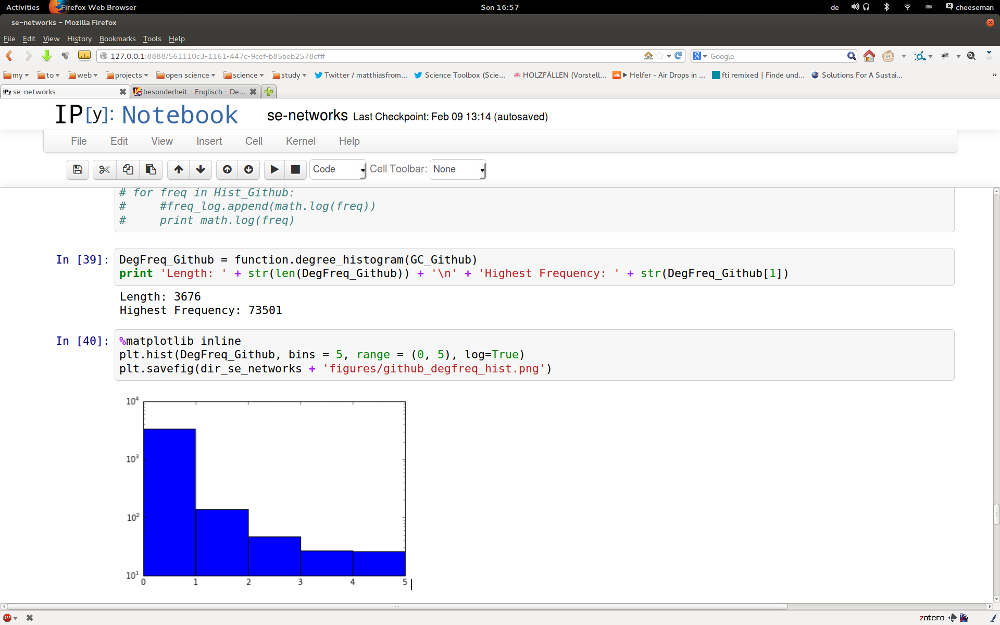
\includegraphics[width=0.8\textwidth]{./images/screenshot-ipython.png}
  \caption{Browser Screenshot from iPython notebook environment}
  \label{fig:screenshot-ipython}
\end{figure}

\subsection{Preprocessing}
\label{sub:preprocessing}

The KONECT data is well structured and has not a lot of additional attributes, so there isn't much preprocessing of the data itself necessary. 
But, because of computational reasons, both networks are way to big to get calculate (shortest path) or the projected in a reasonable amount of time and some calculations need a connected component.

To solve these problems the giant component (largest connected component = lcc) was used for expensive calculations. Sometimes even the second largest connected component was used (2nd lcc), because the giant component still was too big (e. g. shortest path, betwenness centrality, closeness centrality). As table \ref{tab:github-graphs} and \ref{tab:dbpedia-graphs} show, the subgraphs (components) differ a lot in structure and key metrics from the parent graph. It is important to distinguish in the analysis between which graph was used to make right conclusion. 

\begin{table}[h!]
  \begin{center}
    \begin{tabular}{rrrrrr}
      \toprule
      Graph & Users & Projects & Nodes & Edges & Avg. Degree \\
      \midrule
             Parent Graph & 56.519 & 120.867 & 177.386 & 440.237 & 4,96 \\
             Giant Component & 39.845 & 99.907 & 139.752 & 417.361 & 5,97 \\
             2nd lcc & 3 & 42 & 544.947 & 580.231 & 2,12 \\
    \end{tabular}
  \end{center}
  \caption{Properties of GitHub graphs}
  \label{tab:github-graphs}
\end{table}

\begin{table}[h!]
  \begin{center}
    \begin{tabular}{rrrrrr}
      \toprule
      Graph & Entitites & Countries & Nodes & Edges & Avg. Degree \\
      \midrule
             Parent graph & 548.077 & 2.445 & 550.522 & 584.947 & 2,12 \\
             Giant component & 543.589 & 1.358 & 544.947 & 580.231 & 2,12 \\
             2nd lcc & 337 & 1 & 338 & 337 & 1,99 \\
    \end{tabular}
  \end{center}
  \caption{Properties of dbpedia graphs}
  \label{tab:dbpedia-graphs}
\end{table}

The difference of key metrics continues and intensifies through the projection, as the strong increase of edges and the average degree (see table \ref{tab:projected-graphs}) in the dbpedia graph show. For the github graph it was a user-user projection, for the dbpedia an entitie-entitie projection of the 2nd lcc graph. The high degree of dbpedia lies in the very dense and easy structure of only one country connected to 338 entities in the bipartite graph.

\begin{table}[h!]
  \begin{center}
    \begin{tabular}{rrrr}
      \toprule
      Graph & Nodes & Edges & Avg. Degree \\
      \midrule
             Projected GitHub & 3 & 3 & 2,00 \\
             Projected dbpedia & 337 & 56.616 & 336,00 \\
    \end{tabular}
  \end{center}
  \caption{Properties of projected graphs}
  \label{tab:projected-graphs}
\end{table}

As last step, the graphs are tested if the components are connected and if isolated nodes exist.

\subsection{Degree}
\label{sub:degree}

Degree distribution is one of the most important centrality measurements. The whole graphs of both data sets were used for the calculation. As result, the degree distribution was more dense in the low area of the dbpedia network as in Github (see figure \ref{fig:degree-centrality}). This shows, that the average contribution on github is higher than the average number of connections from dbpedia entities to countries, what sounds fair right.

\begin{figure}[h!]
  \centering
  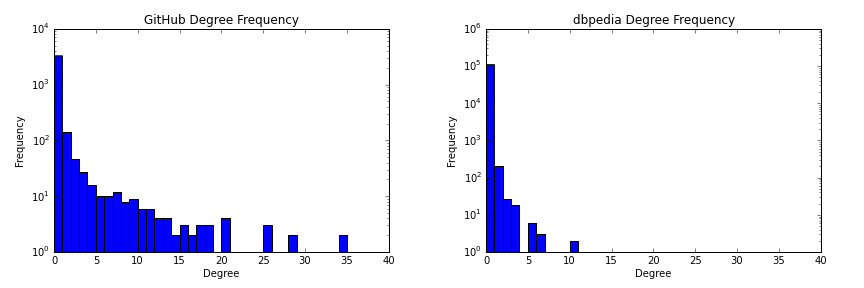
\includegraphics[width=1\textwidth]{./images/degree-centrality.png}
  \caption{Degree distribution on a log-lin scale. The left shows the github network, on the right is dbpedia}
  \label{fig:degree-centrality}
\end{figure}

\subsection{Shortest Path}
\label{sub:shortest-path}

Shortest Path describes the shortest possible way between two nodes. To get the average shortest path of a graph, every possible connection between all nodes have to be computed and divided by the number of paths. Because of the high computational costs for this, the second largest connected components are used. As a result, the github network has slightly higher average shortest path (2,11) than dbpedia (1,99).

\subsection{Clustering}
\label{sub:clustering}

Clustering tells about the density of the graph. This is a very imporant measure for bipartite networks and their projections \citep{latapy_basic_2008}. For the analysis the 2nd lcc network was used, because of computational costs. The average clustering coefficient of the simple dbpedia graph with only one country shows the expected high clustering of the related entities. In general, the clustering coefficients of a projected graph should be much higher than of the original bipartite one. In this case, due to of the very untypical structure of the bipartite networks, this effect can not be seen.

\begin{table}[h!]
  \begin{center}
    \begin{tabular}{rr}
      \toprule
      Graph & Avg. clustering coefficient \\
      \midrule
             Github all & 0,90 \\
             Github users & 0,18 \\
             Github projects & 0,95 \\
             Github projected & 1 \\
             dbpedia all & 1,0 \\
             dbpedia entities & 1.00 \\
             dbpedia countries & 0.00 \\
             dbpedia projected & 1 \\
    \end{tabular}
  \end{center}
  \caption{Clustering coefficients}
  \label{tab:clustering}
\end{table}

\subsection{Diameter}
\label{sub:diameter}

Diameter is the longest of all shortest paths in a network. Because of the underlying cost expensive shortest path algorithm, again, the 2nd lcc network was used. The github network has a diameter of 4, the dbpedia one of 2.

%%%%%%%%%%%%%%%%
%  CONCLUSION  %
%%%%%%%%%%%%%%%%

\section{Conclusion}
\label{sec:conclusio}

The study of networks is still in it's beginning, and so is the research on bipartite networks. A lot of ideas come up for research on 1) weighting algorithms of projections, 2) specialization in the needs of visualization \citep{schulz_visual_2008} and 3) new measurements specifically for bipartite networks and further research on the existing ones. To make knowledge easier transferable, comparability of studies across disciplines and fields should be strived for \citep{piepenbrink_methodological_2013}.

The impression of the first work with iPython was very good. Together with matplotlib it makes a documented, sequencial, integrated and open workflow easily possible. The computation itself proved to be challenging. Networkx is easy to use but the drawing functions are very scarse and need more specific layouts. iGraph looks like a good alternative for this. Also some issues with algorithms occured, maybe failure on my side, maybe bugs. Another problem was typical for large-scale real world networks: the computational costs were huge and not manageable by normal IT-infrastructure, like a standard laptop. For this parallel computing would be necessary.

In the analysis, much more in detail could be done: Comparing the measurements of the two node sets with one another, or comparing it with random graphs for example.

All in all, many questions arose for further investigations on bipartite networks, which would be very helpful to understand network theory in general and the specifics of bipartite networks in particular.

%%%%%%%%%%%%%%
%  OPENNESS  %
%%%%%%%%%%%%%%

\section{Openness}
\label{sec:openness}

\subsection{Copyright}
\label{sub:copyright}

This work is licensed under the Creative Commons Attribution 3.0 AT license\footnote{\url{https://creativecommons.org/licenses/by/3.0/at/}}.

\begin{flushleft}
  
\includegraphics[width=0.14\textwidth]{./images/cc-by.png}
\end{flushleft}

All generated code, content and figures are online freely available on the se-networks GitHub repository\footnote{\url{https://github.com/skasberger/se-networks}} and compatible with the OpenDefinition\footnote{\url{http://opendefinition.org/}}. The sourcecode is licensed under the MIT license\footnote{\url{http://opensource.org/licenses/MIT}}, figures and text under the Creative Commons Attribution 3.0 AT license.\\

\subsection{openscienceASAP}
\label{sub:openscienceASAP}

An own webpage\footnote{\url{http://openscienceasap.org/education/courses/se-networks/}} was created for the Networks Seminar at openscienceASAP\footnote{\url{http://openscienceasap.org}} to collect all informations and works on one central page.
\begin{flushleft}
  
\includegraphics[width=0.3\textwidth]{./images/openscienceASAP-logo.png}
\end{flushleft}

\subsection{Other Sources}
\label{sub:foreign-data-sources}

\begin{itemize}
\item bipartite network dbPedia from KONECT (CC BY-SA) \url{http://konect.uni-koblenz.de/networks/dbpedia-country} \citep{konect:2014:dbpedia-country}
\item bipartite network GitHub from KONECT (CC BY-SA) \url{http://konect.uni-koblenz.de/networks/github} \citep{konect:2014:github}
\end{itemize}

%%%%%%%%%%%%%%%%
%  REFERENCES  %
%%%%%%%%%%%%%%%%

\newpage

\section{Bibliography}
\label{sec:bibliography}
\printbibliography

%%%
%%% end main document
%%%
%%%%%%%%%%%%%%%%%%%%%%%%%%%%%%%%%%%%%%%%%%%%%%%%%%%%%%%%%%%%%%%%%%%%%%%%%%%%%%%%

% \appendix  %% include it, if something (bibliography, index, ...) follows below

%%%%%%%%%%%%%%%%%%%%%%%%%%%%%%%%%%%%%%%%%%%%%%%%%%%%%%%%%%%%%%%%%%%%%%%%%%%%%%%%
%%%
%%% bibliography
%%%
%%% available styles: abbrv, acm, alpha, apalike, ieeetr, plain, siam, unsrt
%%%
% \bibliographystyle{plain}

%%% name of the bibliography file without .bib
%%% e.g.: literatur.bib -> \bibliography{literatur}
% \bibliography{FIXXME}

\end{document}
%%% }}}
%%% END OF FILE
%%%%%%%%%%%%%%%%%%%%%%%%%%%%%%%%%%%%%%%%%%%%%%%%%%%%%%%%%%%%%%%%%%%%%%%%%%%%%%%%
%%% Notice!
%%% This file uses the outline-mode of emacs and the foldmethod of Vim.
%%% Press 'zi' to unfold the file in Vim.
%%% See ':help folding' for more information.
%%%%%%%%%%%%%%%%%%%%%%%%%%%%%%%%%%%%%%%%%%%%%%%%%%%%%%%%%%%%%%%%%%%%%%%%%%%%%%%%
%% Local Variables:
%% mode: outline-minor
%% OPToutline-regexp: "%% .*"
%% OPTeval: (hide-body)
%% emerge-set-combine-versions-template: "%a\n%b\n"
%% End:
%% vim:foldmethod=marker
